\documentclass[a4paper]{report}
\usepackage[spanish]{babel}
\selectlanguage{spanish}
\usepackage[utf8]{inputenc}
\usepackage[T1]{fontenc}
\usepackage{pdfpages}
\usepackage[a4paper,top=2cm,bottom=2cm,left=2cm,right=2cm]{geometry}
\usepackage{amsmath, amsthm, amsfonts}
\usepackage{graphicx}
\usepackage{minitoc}
\usepackage{color}
\usepackage{listings}
\usepackage{hyperref}
\usepackage{multicol}
\usepackage{float}
\usepackage{array}
\usepackage[none]{hyphenat}

\hypersetup{
    colorlinks=true, % make the links colored
    linkcolor=black, % color TOC links in blue
    urlcolor=red, % color URLs in red
    linktoc=all % 'all' will create links for everything in the TOC
}

\lstset{
basicstyle=\ttfamily,
captionpos=b,
frame=single,
texcl=true
}

\def\blankpage{%
      \clearpage%
      \thispagestyle{empty}%
      \addtocounter{page}{0}%
      \null%
      \clearpage}
    
\title{Desarrollo de la Lógica Proposicional y de Primer Orden bajo el paradigma funcional y la orientación Web.}
\author{Víctor Ramos González\\\\
   Tutor: Fernando Sancho Caparrini\\
   \textit{Ciencias de la Computación e Inteligencia Artificial}\\
   E.T.S. Ingeniería Informática\\
   Universidad de Sevilla\\
  \vspace{8cm}
  \date{Septiembre 2020}
}

\newcolumntype{P}[1]{>{\centering\arraybackslash}p{#1}}



\setlength{\parskip}{1em} 
 
\sloppy
\begin{document}

\renewcommand{\tablename}{Tabla}

\dominitoc

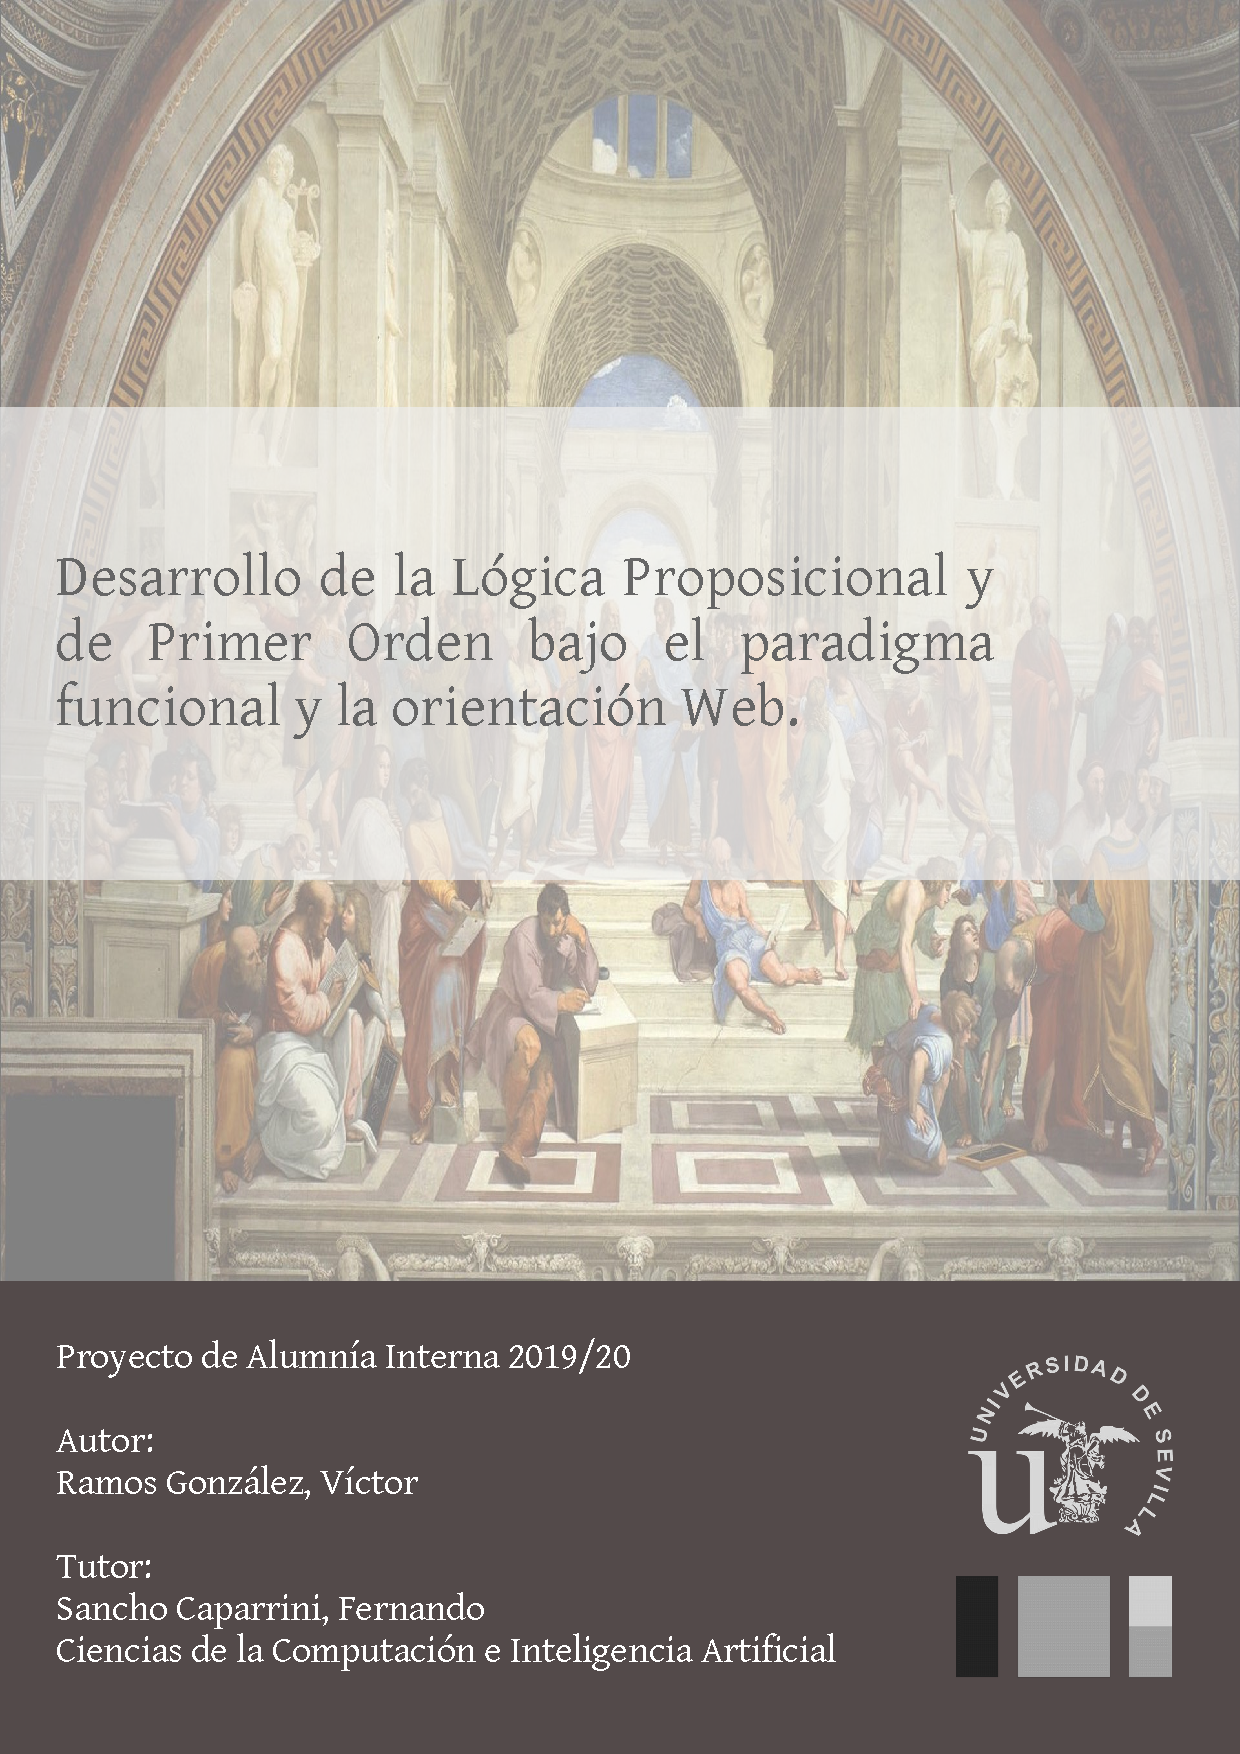
\includepdf[pages={1}]{archivos/titlepage.pdf}


\blankpage

\maketitle

\begin{abstract}

El proyecto aborda los conceptos y algoritmos básicos de la Lógica Proposicional y la Lógica de primer, desde un punto de vista implementativo a través de un lenguaje encuadrado en el paradigma funcional (Elm).

El proyecto, basado en la asignatura de Lógica Informática, busca una doble finalidad, por un lado servir como una somera introducción a la programación declarativa al mismo que tiempo que proporcionar al alumnado  herramientas intuitivas y de sencillo uso en la realización de los ejercicios que apoyen los contenidos teóricos que se desarrollan en dicha asignatura.
\end{abstract}

\tableofcontents

\newpage


\chapter{Introducción. Objetivos y organización del proyecto}
\renewcommand{\mtctitle}{}
\mtcskip
\minitoc
\newpage

\section{Introducción}

Tras haber cursado la asignatura de Lógica Informática con el profesor D. Fernando Sancho Caparrini, director de este proyecto, se despertó mi gusto por la Teoría de la Lógica Matemática y Computacional. Aunque desde el punto de vista teórico la asignatura presentaba los contenidos de forma completa y con total formalismo y corrección, los profesores encargados de la misma pretendían darle a la misma un enfoque más práctico de manera que estos nuevos contenidos sirvieran como complemento a los conceptos formales presentados teóricamente.


\section{Objetivos del proyecto}
El proyecto persigue un doble objetivo,

\section{Estructura del proyecto}

El proyecto se estructará en 2 partes fundamentales:

\subsection{Módulos funcionales}

Se implementan distintos módulos, que se describen detalladamente a lo largo del proceso, en el que se desarrollarán las estructuras y métodos necesarios para abordar los algoritmos vistos en la asignatura.

\subsection{Interfaz gráfica}

\chapter{LP I. Sintaxis y Semántica}
\renewcommand{\mtctitle}{}
\mtcskip
\minitoc
\newpage
\section{Introducción. Descripción general del capítulo}

\textit{TO DO}

\newpage
\section{Módulo SintaxSemanticsLP}

En este primer capítulo vamos a estudiar, desde un punto de vista práctico, a través de las implementaciones, los distintos elementos que conforman la Lógica Proposicional, esto es la Síntaxis y la Semántica que se han presentado en los fundamentos teóricos.

\subsection{Aspectos Sintácticos}

\subsubsection{Átomo y Fórmula Proposicional}

Recordemos que las expresiones están formadas por símbolos proposicionales, organizados en átomos (expresiones básicas) y relaciones entre ellas (conectivas), de acuerdo a esto, podemos definir un símbolo proposicional como una cadena de texto:\\

\begin{lstlisting}[caption={Definición de Símbolo Proposicional como alias de String.}]
type alias PSymb = String 
\end{lstlisting}

Y las conectivas lógicas como categorías del tipo recursivo \textit{Prop}, de forma que:\\

\begin{lstlisting}[caption= Definición del tipo Prop (Proposición).]
type Prop = Atom PSymb
          | Neg Prop
          | Conj Prop Prop
          | Disj Prop Prop
          | Impl Prop Prop
          | Equi Prop Prop
\end{lstlisting}

Esto nos permite definir todas las fórmulas proposicionales que se pueden formar, algunos ejemplos: \\

\begin{multicols}{3}
\begin{itemize}
\item[(a)] $ (p \wedge q) \vee (p \wedge r)$
\item[(b)] $ (p \wedge r) \vee (\neg p \wedge q) \rightarrow \neg q$
\item[(c)] $(p \leftrightarrow q) \wedge (p \rightarrow \neg q) \wedge p$
\end{itemize}
\end{multicols}

\begin{lstlisting}[caption= Ejemplos de definición de fórmulas proposicionales.]
a = Disj (Conj (Atom "p") (Atom "q")) (Conj (Atom "p") (Atom "r"))
    
b = Impl 
        (Disj 
            (Conj (Atom "p") (Atom "r")) 
            (Conj (Neg (Atom "p")) (Atom "q"))
        ) 
        (Neg (Atom "q"))

c = Conj 
        (Conj 
            (Equi (Atom "p") (Atom "q")) 
            (Impl (Atom "p") (Neg (Atom "q"))) 
        (Atom "p")
\end{lstlisting}

Como se puede apreciar, escribir las fórmulas de esta forma puede resultar una tarea ardua y propensa a errores, por eso, como mostraremos más adelante, se ha desarrollado un parser que nos permite escribir de forma más cómoda, sintética y visual las fórmulas. Aunque aquí no influyen las reglas de asociación vistas en los fundamentos teóricos, ya que dicho orden viene dado por el propio orden de aplicación, sí hemos de tenerlas en cuenta a la hora de realizar el parser. 

\subsubsection{Conjuntos de fórmulas}

Definidas las fórmulas proposicionales, definiremos los conjuntos de fórmulas como listas de fórmulas proposicionales de manera que una misma fórmula puede aperecer varias veces en el conjunto. De esta forma: \\

\begin{lstlisting}[caption= Definición de Conjunto de Fórmulas como Lista de Fórmulas Proposicionales]
type alias PropSet = List Prop
\end{lstlisting}

\subsection{Aspectos Semánticos}
\subsubsection{Interpretaciones y Valor de verdad de fórmulas proposicionales. }

Una vez provista la sintaxis, pasamos a desarrollar la semántica de la Lógica Proposicional. Aunque en secciones futuras mostraremos la implementación del parser, por ahora vasta conocer la estructura de las fórmulas para hacer abordable la implementación que se ha llevado a cabo de la semática del lenguaje de la lógica de proposiciones.

Como ya se ha comentado, y explicado en los fundamentos teóricos, hemos de abordar la interpretación de las fórmulas, y para ello hemos de crear las estructuras necesarias que nos permitan representar interpretaciones, esto es, definir los símbolos proposicionales con valor de verdad 1 y aquellos con valor 0. Para ello, hemos elegido una representación "dispersa" de manera que una interpretación corresponde a una lista de símbolos proposicionales que son los que son considerados verdaderos, los términos que no aparecen en la lista serán considerados como falsos.\\

\begin{lstlisting}[caption= Definición de Interpretación como Lista de Símbolos Proposicionales]
type alias Interpretation = List PSymb
\end{lstlisting}

De esta forma podemos definir, de forma sencilla la evaluación de las fórmulas, de forma que el valor de verdad de un símbolo se reduce a la pertenencia del mismo a la lista de interpretación, de esta forma, podemos, dada la estructura recursiva definida para las fórmulas proposicionales, establecer una función, tambieén recursiva, que nos permite evaluar las mismas:

\begin{itemize}
\item (\textit{Caso base}) Una fórmula atómica será verdadera si y sólo si el símbolo proposicional pertenece a la lista de interpretación.

\item (Casos recursivos) Según la clase de fórmula:
\begin{itemize}
\item La negación de una fórmula será verdadera respecto de una interpretación si y sólo si la evaluación de la fórmula es falsa.
\item La conjunción de dos fórmulas proposicionales será verdadera respecto de una interpretación si y sólo si la evaluación de ambas fórmulas respecto de dicha evaluación es verdadera.
\item La disyunción de dos fórmulas proposicionales será verdadera será verdadera respecto de una interpretación si y sólo si alguna de las evaluaciones de las dos fórmulas es evaluada verdadera respecto de dicha interpretación.
\item La implicación será verdadera respecto de una interpretación si y sólo si o la evaluación del antecedente es evaluado falso respecto de dicha interpretación o el consecuente es evaluado verdadero respecto de la misma.
\item La equivalencia será verdadera respecto de una interpretación si y sólo si la evaluación del antecedente coincide con la evaluación del consecuente.\\
\end{itemize} 

\newpage
\begin{lstlisting}[caption= Función de evaluación de las fórmulas proposicionales]
valuation : Prop -> Interpretation -> Bool
valuation pr i =
    case pr of
        Atom p -> List.member p i
        Neg p -> not (valuation p i)
        Conj p q -> valuation p i &&  valuation q i
        Disj p q ->   valuation p i ||  valuation q i
        Impl p q ->   not (valuation p i) ||  valuation q i
        Equi p q ->   valuation (Impl p q) i &&  valuation (Impl q p) i
\end{lstlisting}
\end{itemize}

\subsubsection{Modelos (tablas de verdad, satisfactibilidad y validez lógica)}

Desde el punto de vista teórico las tablas de verdad corresponden a estructuras que reflejan el valor de verdad de una fórmula proposicional respecto de cada una de las posibles interpretaciones posibles para la fórmula. Entonces, para poder construir la tabla de verdad, primero hemos de calcular todas las interpretaciones posibles, que, dada la definición que hemos proporcionado para las interpretaciones, correspondería a todos los conjuntos posibles (\textit{powerset}) que podríamos construir con los símbolos proposicionales que aparecen en la fórmula. Así:\\

\begin{lstlisting}[caption= Función para extraer los símbolos proposicionales que intervienen en una fórmula]
symbInProp : Prop -> Set PSymb

symbInProp f=
    case f of
        Atom p -> Set.singleton p
        Neg p -> symbInProp p
        Conj p q -> Set.union (symbInProp p ) (symbInProp q)
        Disj p q -> Set.union (symbInProp p ) (symbInProp q)
        Impl p q -> Set.union (symbInProp p ) (symbInProp q)
        Equi p q -> Set.union (symbInProp p ) (symbInProp q)
\end{lstlisting}

\begin{lstlisting}[caption= Función para extraer las posibles interpretaciones para una fórmula propsicional]
allInterpretations : Prop -> List Interpretation
allInterpretations x =  Aux.powerset <| List.sort <| Set.toList 
                                                         <| symbInProp x
\end{lstlisting}

De esta forma podemos expresar la tabla de verdad como una lista de tuplas en las que el primer elemento corresponde a la interpretación y el segundo corresponde a la evaluación de la fórmula respecto de dicha valoración:\\

\begin{lstlisting}[caption= Función para la construcción de la tabla de verdad de una fórmula]
truthTable : Prop -> List (Interpretation, Bool)
truthTable x = List.map (\xs ->  (xs,valuation x xs)) <| allInterpretations x
\end{lstlisting}

Una vez estudiado lo anterior, los modelos corresponden a las interpretaciones que son evaluadas verdaderas, esto es, de las posibles interpretaciones aquellas hacen la fórmula verdadera. Aquellas interpretaciones que hacen la fórmula falasa se denominan contramodelos. Así:\\

\newpage
\begin{lstlisting}[caption= Función para el cálculo de los modelos de una fórmula proposicional]
models : Prop -> List Interpretation
models x = List.filter (\y -> valuation x y) (allInterpretations x)

countermodels : Prop -> List Interpretation
countermodels x = List.filter (\y -> not (valuation x y)) 
                                               (allInterpretations x)
\end{lstlisting}

Definidos los modelos, podemos así mismo definir (funcionalmente) los conceptos de satisfactibilidad y validez, de forma que:

\begin{itemize}
\item Una fórmula es satisfactible si posee al menos un modelo.
\item Una fórmula es lógicamente válida o tautología si toda interpretación es modelo de la fórmula.
\item Una fórmula es insatisfactible o contradicción si no posee ningún modelo.
\end{itemize}

De esta forma:

\begin{lstlisting}[caption={Funciones de Satisfactibilidad, Validez e Insatisfactibilidad}]
satisfactibility : Prop -> Bool
satisfactibility x = List.any (\xs-> valuation x xs) (allInterpretations x)

validity : Prop -> Bool
validity x = List.all (\xs-> valuation x xs) (allInterpretations x)

insatisfactibility : Prop -> Bool
insatisfactibility x = not (satisfactibility x)
\end{lstlisting}

\subsubsection{Conjuntos de Fórmulas. Modelos, Consistencia, Validez y Consecuencia Lógica}

Vista la satisfactibilidad, modelos, etc. aplicadas a una fórmula, pasamos a desarrollar los métodos necesarios para el estudio de la satisfactibilidad (consistencia) , inconsistencia en conjuntos de fórmulas. Ahora los modelos del conjunto de fórmulas corresponden a las interpretaciones tales que hacen verdaderas todas las fórmulas del conjunto. Para obtener los modelos hemos, al igual que en el caso de las fórmulas, obtener el conjunto de símbolos proposicionales y a partir de estos el conjunto de todas las posibles interpretaciones. De forma que:\\

\begin{lstlisting}[caption={Modelos y contramodelos en conjuntos de fórmulas proposicionales}]
setSymbols : List Prop -> Set PSymb
setSymbols xs = 
    List.foldr (\x acc -> Set.union acc (symbInProp x)) Set.empty xs

allSetInterpretations : List Prop -> List Interpretation
allSetInterpretations xs = Aux.powerset <| Set.toList <| setSymbols xs
    
isSetModel : List Prop -> Interpretation -> Bool
isSetModel xs i =  List.all (\x -> valuation x i) xs

allSetModels : List Prop -> List Interpretation
allSetModels xs = List.filter (isSetModel xs) (allSetInterpretations xs)

allSetCounterModels : List Prop -> List Interpretation
allSetCounterModels xs = 
    List.filter (\x -> not(isSetModel xs x)) <| allSetInterpretations xs
\end{lstlisting}


De forma que ahora, es sencillo, comprobar la consistencia de un conjunto a partir de la definición: \textit{`Un conjunto es consistente si posee, al menos, un modelo. En caso contrario es inconsistente'}\\

\begin{lstlisting}[caption={Consistencia e Inconsistencia en Conjuntos Proposicionales}]
isConsistent : List Prop -> Bool
isConsistent xs = 
    List.any (\x -> isSetModel xs x) <| allSetInterpretations xs
    
isInconsistent: List Prop -> Bool
isInconsistent xs = not(isConsistent xs)
\end{lstlisting}

Por último nos queda definir el concepto de consecuencia lógica. Acudiendo a la definición: \textit{`Una fórmula es consecuencia lógica de un conjunto de fórmulas si y sólo si todo modelo del conjunto es también modelo de la fórmula'}, pero también \textit{`Una fórmula es consecuencia lógica de un conjunto de fórmulas si la unión del conjunto y el conjunto formado por la negación del la fórmula es inconsistente.'}. De esta forma podemos plantear dos desarrollos alternativos:\\

\begin{lstlisting}[caption={Consecuencia Lógica}]
isConsecuence : List Prop -> Prop -> Bool
isConsecuence xs x = List.all (\y -> valuation x y) <| allSetModels xs

isConsecuence : List Prop -> Prop -> Bool
isConsecuence xs x = isInconsistent (xs ++ [Neg x])
\end{lstlisting}

\subsection{Código del módulo y resumen de funciones}
\subsubsection{Código del módulo}
\begin{lstlisting}[caption={Módulo SintaxSemanticsLP}]
module Modules.SintaxSemanticsLP exposing (
    PSymb, Prop, Interpretation,PropSet,
    valuation, truthTable, models, countermodels, satisfactibility, 
    validity, insatisfactibility, isSetModel, allSetModels, 
    allSetCounterModels, isConsistent, isInconsistent, isConsecuence)

import List
import Set
import Modules.AuxiliarFunctions as Aux 


-----------
-- TYPES --
-----------
type alias PSymb = String 

type Prop = Atom PSymb
          | Neg Prop
          | Conj Prop Prop
          | Disj Prop Prop
          | Impl Prop Prop
          | Equi Prop Prop

type alias Interpretation = List PSymb
type alias PropSet = List Prop



-------------
-- METHODS --
-------------

valuation : Prop -> Interpretation -> Bool
valuation pr i =
    case pr of
        Atom p -> List.member p i
        Neg p -> not (valuation p i)
        Conj p q -> valuation p i &&  valuation q i
        Disj p q ->   valuation p i ||  valuation q i
        Impl p q ->   not (valuation p i) ||  valuation q i
        Equi p q ->   valuation (Impl p q) i &&  valuation (Impl q p) i

symbInProp : Prop -> Set.Set PSymb

symbInProp f=
    case f of
        Atom p -> Set.singleton p
        Neg p -> symbInProp p
        Conj p q -> Set.union (symbInProp p ) (symbInProp q)
        Disj p q -> Set.union (symbInProp p ) (symbInProp q)
        Impl p q -> Set.union (symbInProp p ) (symbInProp q)
        Equi p q -> Set.union (symbInProp p ) (symbInProp q)

allInterpretations : Prop -> List Interpretation
allInterpretations x =  
    Aux.powerset <| List.sort <| Set.toList <| symbInProp x

truthTable : Prop -> List (Interpretation, Bool)
truthTable x = List.map (\xs ->  (xs,valuation x xs)) <| allInterpretations x

models : Prop -> List Interpretation
models x = List.filter (\y -> valuation x y) (allInterpretations x)

countermodels : Prop -> List Interpretation
countermodels x =
    List.filter (\y -> not(valuation x y)) (allInterpretations x)

satisfactibility : Prop -> Bool
satisfactibility x = List.any (\xs-> valuation x xs) (allInterpretations x)
validity : Prop -> Bool
validity x = models x== allInterpretations x
insatisfactibility : Prop -> Bool
insatisfactibility x = List.isEmpty (models x)

setSymbols : List Prop -> Set.Set PSymb
setSymbols xs = 
    List.foldr (\x acc -> Set.union acc (symbInProp x)) Set.empty xs

allSetInterpretations : List Prop -> List Interpretation
allSetInterpretations xs = Aux.powerset <| Set.toList <| setSymbols xs

isSetModel : List Prop -> Interpretation -> Bool
isSetModel xs i =  List.all (\x -> valuation x i) xs

allSetModels : List Prop -> List Interpretation
allSetModels xs = List.filter (isSetModel xs) (allSetInterpretations xs)



allSetCounterModels : List Prop -> List Interpretation
allSetCounterModels xs = 
    List.filter (\x -> not(isSetModel xs x)) <| allSetInterpretations xs

isConsistent : List Prop -> Bool
isConsistent xs = 
    List.any (\x -> isSetModel xs x) <| allSetInterpretations xs

isInconsistent: List Prop -> Bool
isInconsistent xs = not(isConsistent xs)

isConsecuence : List Prop -> Prop -> Bool
--isConsecuence xs x = List.all (\y -> valuation x y) <| allSetModels xs
isConsecuence xs x = isInconsistent (xs ++ [Neg x])
\end{lstlisting}


\subsubsection{Funciones disponibles}

\begin{table}[H]
\centering
\begin{tabular}{p{3cm} p{13.2cm}}
\hline
Tipo & Descripción\\
\hline
\hline
\textit{PSymb} & Alias de \textit{String}. Representa los símbolos proposicionales.\\
\hline
\textit{Prop}& Representa a las proposiciones o fórmulas proposicionales. Posee varios constructores según el tipo de fórmula proposicional: (\textit{Atom, Neg, Conj, Disj, Impl, Equi}).\\
\hline
\textit{Interpretation}& Alias de \textit{List PSymb}. Representa una interpretación, de forma que se consideran verdaderos los símbolos proposicionales que aparecen en la lista, y falsos aquellos que no aparecen.\\
\hline
\textit{PropSet}& Alias de \textit{List Prop}. Representa conjuntos de fórmulas.\\
\hline
\end{tabular}
\caption{Módulo SintaxSemanticsLP I. Tipos}
\vspace{0.5cm}
\begin{tabular}{p{3cm} p{13.2cm}}
\hline
Método & Descripción\\
\hline
\hline
\textit{valuation}& \textit{valuation: Prop -> Interpretation -> Prop}\\
& Calcula el valor de verdad de una proposición según la interpretación dada.\\
\hline
\textit{truthTable}& \textit{truthTable: Prop -> List (Interpretation, Bool
)}\\
& Calcula la tabla de verdad asociada a una fórmula proposicional, devolviéndola como una lista de pares (Interpretación, Valoración).\\
\hline
\textit{models}& \textit{models: Prop -> List Interpretation}\\
& Calcula los modelos de una fórmula proposicional.\\
\hline
\textit{countermodels}& \textit{countermodels: Prop -> List Interpretation}\\
& Calcula los contramodelos de una fórmula proposicional.\\
\hline
\textit{satisfactibility}& \textit{satisfactibility: Prop -> Bool}\\
& Decide si una fórmula proposicional es satisfactible o no.\\
\hline
\textit{validity}& \textit{validity: Prop -> Bool}\\
& Decide si una fórmula proposicional es tautología o no.\\
\hline
\textit{insatisfactibility}& \textit{insatisfactibility: Prop -> Bool}\\
& Decide si una fórmula proposicional es insatisfactible o no.\\
\hline
\textit{isSetModel}& \textit{isSetModel: List Prop -> Interpretation ->Bool}\\
& Decide si una interpretación es modelo de un conjunto de fórmulas proposicionales o no.\\
\hline
\textit{allSetModels}& \textit{allSetModels: List Prop -> List Interpretation}\\
& Calcula los modelos asociados a un conjunto de fórmulas proposicionales.\\
\hline
\textit{allSetCounterModels}& \textit{allSetCounterModels: List Prop -> List Interpretation}\\
& Calcula los contramodelos asociados a un conjunto de fórmulas proposicionales.\\
\hline
\textit{isConsistent}& \textit{isConsistent: List Prop -> Bool}\\
& Decide si un conjunto de fórmulas proposicionales es consistente o no.\\
\hline
\textit{isInconsistent}& \textit{isInconsistent: List Prop -> Bool}\\
& Decide si un conjunto de fórmulas proposicionales es inconsistente o no.\\
\hline
\textit{isConsecuence}& \textit{isConsecuence: List Prop -> Prop -> Bool}\\
& Decide si una fórmula es consecuencia lógica de un conjunto de fórmulas proposicionales.\\
\hline
\end{tabular}
\caption{Módulo SintaxSemanticsLP II. Funciones}
\end{table}

\newpage

\section{LP Parser I. Módulo LP\_Parser}

En la sección anterior se ha mostrado el desarrollo necesario para la definición de las fórmulas proposicionales, pero como ya comentamos realizarlo a través de los constructores puede ser una tarea pesada por ello vamos a definir un lenguaje (a través de un Parser), que nos permita escribir las fórmulas de forma más natural, utilizando operadores infijos (\textit{LP\_Parser}) o utilizar operadores \textit{Big}, que nos permitan expresar la conjunción/disyunción de muchas fórmulas análogas sin necesidad de tener que escribirlas una a una (\textit{LPBig\_Parser})

En esta sección vamos a definir un Parser que nos permita trasladar la definición de las fórmulas desde un lenguaje mucho más cercano al lenguaje de escritura de la lógica a los constructores que se han definido en el módulo anterior, y con los que trabajaran los distintos algoritmos que se van a ir desarrollando. Para ello vamos a hacer uso de algunas herramientas que nos provee Elm para la construcción del Parser.

Vamos a definir las reglas asociadas a nuestro lenguaje:

\begin{itemize}
\item Las variables proposicionales (símbolos proposicionales) han de comenzar por una letra minúscula y han de contener exclusivamente caracteres alfanuméricos.

\item Cada una de las fórmulas debe ir escrita entre paréntesis. Aunque en nuestro lenguaje esto es fundamental, la función parseadora de fórmulas ya incorpora estos paréntesis a la cadena leída, por lo que no es necesario que se escriban explícitamente los paréntesis.

\item Se admiten los siguientes operadores:

\begin{table}[H]
\centering
\begin{tabular}{P{3cm} p{5cm}}
\hline
Operador & Descripción\\
\hline
\hline
¬ & Representa la Negación.\\
\hline
\& & Representa la Conjunción.\\
\hline
| & Representa la Disjunción.\\
\hline
-> & Representa la Implicación.\\
\hline
<-> & Representa la Equivalencia.\\
\hline
\end{tabular}
\caption{LP\_Parser. Operadores Proposicionales}
\end{table}

\item Se admiten espacios (pero no son obligatorios) entre los símbolos proposicionales y los operadores.

\item La prioridad de los operadores viene dada según el orden de prioridad definido por la lógica proposicional, según el orden en el que aparecen en la tabla anterior.

\item Para la definición de conjuntos de fórmulas proposicionales, seguir las reglas anteriores para cada una de las fórmulas, separando éstas por el símbolo \textit{;} .
\end{itemize}

\subsection{Código del módulo y resumen de funciones}

\subsubsection{Código del módulo}

\begin{lstlisting}[caption={Módulo LP\_Parser}, mathescape=true]

module Modules.LP_Parser exposing(parserProp, parserPropSet)

import Char
import Set
import String
import Maybe

import Parser exposing (Parser, run, variable, oneOf, succeed, spaces, (|.), 
                        (|=), symbol, lazy, andThen)

import Modules.SintaxSemanticsLP exposing (PSymb, Prop, atomProp, negProp, 
                                           conjProp, disjProp, implProp, 
                                           equiProp)

parserProp : String -> (Maybe (Prop), String)
parserProp x =
  if x == "" then
        (Maybe.Nothing, "Argument is empty")
  else
    case run lpParser ("(" ++ x ++ ")") of
      
      Ok y-> (Maybe.Just y, "")

      Err y -> (Maybe.Nothing, Debug.toString y)

parserPropSet : String -> List (Maybe(Prop), String)
parserPropSet x =  List.map parserProp <| String.split ";" x

typeVar : Parser PSymb
typeVar =
  variable
    { start = Char.isLower
    , inner = \c -> Char.isAlphaNum c
    , reserved = Set.fromList []
    }

lpParser : Parser Prop
lpParser =
  oneOf 
  [ 
    succeed atomProp
      |. spaces
      |= typeVar
      |. spaces

  , succeed identity 
    |. symbol "("
    |. spaces
    |= lazy(\_ -> expression)
    |. spaces
    |. symbol ")"
    |. spaces  
  
  , succeed negProp
    |.spaces
    |.symbol "$\neg$"
    |.spaces
    |= lazy(\_ -> lpParser)
  ]

expression : Parser Prop
expression =
  lpParser |> andThen (expressionAux [])

type Operator = AndOp | OrOp | ImplOp | EquivOp

operator : Parser Operator
operator = 
    oneOf
    [ Parser.map (\_ -> AndOp) (symbol "&")
    , Parser.map (\_ -> OrOp) (symbol "|")
    , Parser.map (\_ -> ImplOp) (symbol "->")
    , Parser.map (\_ -> EquivOp) (symbol "<->")
    ]

expressionAux : List (Prop, Operator) -> Prop -> Parser Prop
expressionAux revOps expr =
  oneOf
    [ succeed Tuple.pair
        |. spaces
        |= operator
        |. spaces
        |= lpParser
        |> andThen 
             (\(op, newExpr) -> expressionAux ((expr,op) :: revOps) newExpr)
    , lazy (\_ -> succeed (finalize revOps expr))
    ]

finalize : List (Prop, Operator) -> Prop -> Prop
finalize revOps finalExpr =
  case revOps of
    [] ->
      finalExpr

     
    (expr, AndOp) :: otherRevOps ->
      finalize otherRevOps (conjProp expr finalExpr)


    (expr, OrOp) :: (expr2, AndOp) :: otherRevOps ->
      disjProp (finalize ( (expr2, AndOp) :: otherRevOps) expr) finalExpr

    (expr, OrOp) :: otherRevOps ->
      finalize otherRevOps (disjProp expr finalExpr)


    (expr, ImplOp) :: (expr2, AndOp) :: otherRevOps ->
      implProp (finalize ( (expr2, AndOp) :: otherRevOps) expr) finalExpr

    (expr, ImplOp) :: (expr2, OrOp) :: otherRevOps ->
       implProp (finalize ( (expr2, OrOp) :: otherRevOps) expr) finalExpr

    (expr, ImplOp) :: otherRevOps ->
      finalize otherRevOps (implProp expr finalExpr)


    (expr, EquivOp) :: (expr2, AndOp) :: otherRevOps ->
      equiProp (finalize ( (expr2, AndOp) :: otherRevOps) expr) finalExpr

    (expr, EquivOp) :: (expr2, OrOp) :: otherRevOps ->
       equiProp (finalize ( (expr2, OrOp) :: otherRevOps) expr) finalExpr

    (expr, EquivOp) :: (expr2, ImplOp) :: otherRevOps ->
       equiProp (finalize ( (expr2, ImplOp) :: otherRevOps) expr) finalExpr

    (expr, EquivOp) :: otherRevOps ->
      finalize otherRevOps (equiProp expr finalExpr)
      
\end{lstlisting}


En el anexo \textit{A1. El Lenguaje Elm. Parsers} se explica cada una de las funciones del módulo Parser utilizadas en el código anterior.

\subsubsection{Funciones disponibles}

\begin{table}[H]
\centering
\begin{tabular}{p{3cm} p{13.2cm}}
\hline
Método & Descripción\\
\hline
\hline
\textit{parserProp}& \textit{parserProp : String -> (Maybe (Prop), String)}\\
& Recibe una String y devuelve una tupla que contiene una Maybe Prop (Just Prop [si no hay errores] o Nothing [en caso de error], y una String (vacía ("") [si no hay error] o mensaje del error [en caso de error]).\\
\hline
\textit{parserPropSet}& \textit{parserPropSet : String -> List (Maybe(Prop), String)}\\
& Recibe una String y devuelve una lista de tuplas (análogas a las proporcionadas por \textit{parserPropSet}) con cada una de las lecturas de las fórmulas.\\
\hline
\end{tabular}
\caption{Módulo LP\_Parser. Funciones disponibles}
\end{table}

\section{LP Parser II. Módulo LPBig\_Parser}
En la sección anterior desarrollamos un Parser para simplificar la escritura de las fórmulas. En esta vamos a realizar otro Parser que nos va a permitir utilizar los operadores \textit{bigAnd} ($\bigwedge$) y \textit{bigOr} ($\bigvee$), enfocado, principalmente, al modelado de restricciones para CSPs (\textit{Constraint Satisfaction Problems}).

En este caso la complejidad del Parser es más alta, ya que hemos de recojer el conjunto de valores, que participarán en las formulas definida y estarán sujetos a una serie de filtros o condiciones (expresiones aritmetico-booleanas), por tanto hemos de realizar la adaptación de todos estos aspectos. Vamos a tratar de resumir los requisitos más relevantes y mostrar las reglas de sintáctico-semánticas asociadas a este lenguaje, y después veremos el desarrollo que se ha desarrollado de cada uno de los puntos.

\noindent\underline{Reglas Sintáctico-Semánticas}

\begin{itemize}
\item Lo primero que vamos a presentar es la estructura general de las fórmulas con operadores \textit{Big}, a lo largo de la sección iremos desarrollando cada una de las partes de estas expresiones. Mostremos la estructura:
\begin{center} \textit{Operador} \textit{\{Declar. índices\}} \textit{\{Restricc. índices\} }  \textit{Fórmula}\end{center} 

\item \textbf{\textit{Operador}}. Existen 2 posibles operadores, el operador de conjunción múltiple (\textit{BigAnd}), representado mediante el símbolo `\&\_'; y el operador de disyunción múltiple (\textit{BigOr}), representado por el símbolo `|\_'

\item \textbf{\textit{Declaración de índices}}. Corresponde a la declaración de las variables que actuarán de índices de los símbolos proposicionales de las fórmulas. Además hemos de establecer los valores (numéricos enteros) que se permiten para los índices. La sintaxis de estas declaraciones es sencilla, el identificador debe comenzar por el símbolo `\_' y ha de seguir por un secuencia de caracteres alfabéticos (en mayúsculas) y/o dígitos numéricos y seguido, los valores que puede tomar dicha variable. Para ello, se permiten 2 alternativas, declaración por valores o declaración por rango. La declaración por valores consiste en definir los valores concretos que tomará la variable, para ello se da la secuencia de valores entre llaves y separados por comas (ej. \_I$\{1,2,3,4\}$). En la declaración por rango se da el rango de valores en el que se moverá la variable. Para ello se da, entre corchetes, el primer número del rango seguido de \textit{`:'} y seguido del último número del rango (ej \_I$[1:4]$). 

\item \textbf{\textit{Restricción de índices}}. Podemos establecer una restricción (y sólo una) sobre los valores de las variables, que puede afectar a todas (o sólo a algunas) de las variables declaradas. Corresponde a una expresión booleana que modela las posibles restricciones sobre los valores que pueden tomar las variables. Aunque solo se permite una única restricción, esta puede estar formada por varias condiciones, así tenemos distintas estructuras y operadores que podemos utilizar en estas expresiones:

\begin{itemize}
\item \textit{Condiciones}. Establecen posibles restricciones del problema modelado.
\begin{itemize}
\item \underline{Condiciones básicas}. Representan expresamente el valor de verdad de la condición. \textit{`T'} corresponde a \textit{True} y \textit{`F'} corresponde a \textit{False}.

\item \underline{Condiciones comparativas}. Escrita entre corchetes, compara dos expresiones aritméticas. Está compuesta por tres elementos, las expresiones que son comparadas (\textit{LHS} y \textit{RHS}) y el operador comparador, que puede ser uno de \textit{mayor o igual} (>=), \textit{menor o igual} (>=), \textit{mayor que} (>), \textit{igual} (=), \textit{distinto} (!=).\\
\newpage
Las expresiones aritméticas corresponden a una expresión que puede contener valores numéricos enteros, variables de índices, de las previamente declaradas, y/o operadores aritméticos: \textit{suma} (`+'), \textit{diferencia} (`-'), \textit{producto} (`*'), \textit{cociente entero} (`/') y módulo (`\%'). \\

Ejemplo: 
\textrm{\small`\&\_ {\_I[0:7], \_J[0:7]}{T}(p\_I\_J -> \&\_ {\_K[-7:7],\_U[0:7],\_V[0:7]} {[\_K!=0]AND[\_U=\_I+\_K]AND[\_V=\_J-\_K]} ($\neg$ p\_U\_V));'} 

\end{itemize}
\end{itemize}



\end{itemize}





\subsection{Módulo A\_Expressions (Expr. Aritméticas)}
\subsection{Módulo B\_Expressions (Expr. Booleanas)}
\subsection{Módulo LPBig\_Parser}

\section{Módulo LP\_toString}



\chapter{LP II. Tableros Semánticos}
\renewcommand{\mtctitle}{}
\mtcskip
\minitoc
\newpage
\chapter{LP III. Formas Normales y DPLL}
\renewcommand{\mtctitle}{}
\mtcskip
\minitoc
\newpage
\chapter{LP IV. Sistemas Deductivos}
\renewcommand{\mtctitle}{}
\mtcskip
\minitoc
\newpage
\chapter{LP V. Algoritmo de Resolución}
\renewcommand{\mtctitle}{}
\mtcskip
\minitoc
\newpage
\chapter{LP VI. Modelado y Resolución de PSR a través de la LP}
\renewcommand{\mtctitle}{}
\mtcskip
\minitoc
\newpage

\chapter{LPO I. Sintaxis y Semántica}
\renewcommand{\mtctitle}{}
\mtcskip
\minitoc
\newpage
\chapter{LPO II. Tableros Semánticos}
\renewcommand{\mtctitle}{}
\mtcskip
\minitoc
\newpage
\chapter{LPO III. Forma Prenex, Skolem y Teorema de Herbrand}
\renewcommand{\mtctitle}{}
\mtcskip
\minitoc
\newpage
\chapter{LPO V. Algoritmos de Unificación y Resolución}
\renewcommand{\mtctitle}{}
\mtcskip
\minitoc
\newpage
\chapter{LPO VI. Modelado y Resolución de PSR a través de la Lógica de Primer Orden}
\renewcommand{\mtctitle}{}
\mtcskip
\minitoc
\newpage

\end{document}